\section {Information Theory}

Information theory was originally proposed by Claude E. \textbf{Shannon} (\textit{A mathematical theory of communication}, 1948) and his goal was to \textbf{mathematically formalize the concept of information} and, more generally, of \textbf{communication}. In this sense, he didn't want to study a specific communication system, but to develop a \textbf{general} one. 

\subsection{Communication system}
According to his theory, a communication system can be abstracted as follows:

\image{img/channel1}{Communication system}{0.8}

This representation is composed by the following components (notice that there could be some variants):

\begin{itemize}
    \item the \textbf{source} and the \textbf{destination}. Normally, the source starts the communication by sending some pieces of information, while the destination receives the information. These two entities are not necessarily different;
    \item a \textbf{transmitter}, which translates the message language of the source to the one of the channel;    
    \item a \textbf{channel}, which is the medium that allows the transmission of messages between two entities;
    \item the \textbf{noise}, which is an unpredictable phenomenon that can interfere the communication;
    \item a \textbf{receiver}, which translates the message to the language of the destination.
\end{itemize}

\subsection{Information}
Another goal of Shannon's work was both to understand the \textbf{nature of information} and how to \textbf{measure} the amount of information that travels through a channel. In this sense, he distinguished 3 different levels of information:

\begin{enumerate}
    \item \textbf{Symbolic level}, which deals only with the symbols of the message, and it does not consider its semantic (meaning);
    \item \textbf{Semantic level}, which deals with the meaning of the message, so it tries to understand the semantic. It is very complex;
    \item \textbf{Pragmatic level}, which studies how the context affects the meaning of a message and what are the intentions of the speaker.
\end{enumerate}

Classical information theory only deals with symbolic level.

\subsection{Quantifying the information}
Quantifying information refers to the necessity of finding a measure to quantify the \textbf{amount of information} that travels inside the \textbf{channel}. However, firstly, it is necessary to give a definition of information.

Shannon's intuition was based on the connection between the concept of \textit{information} and \textit{probability} of an event. Suppose we have an event $E$ and its associated probability $P(E)$. We can study the information $I(E)$ provided by the event $E$ as follows:

\begin{itemize}
    \item If $P(E) = 1$, the amount of information $I(E)$ provided by event $E$ is 0.
    \item If $P(E) = 0$, the amount of information provided by the event E is $\infty$.
\end{itemize}

In this sense, we understand that the concept of \textit{information} is closely related to concepts as \textbf{uncertainty} and \textbf{surprise}, so in general $I(E)$ can be considered as a function of $P(E)$.

\subsubsection{Shannon function} 
After the premises made so far, we can consider the amount of information $I(E)$ provided by an event $E$ as a function of the probability of the event $E$: $I(E) = f(P(E))$, which can be represented as follows:

\image{img/ieFunction1}{Possible configurations of function $I(E)$.}{0.5}

It is important to notice that we do not know how $I(E)$ behaves in the middle but we can definitely state that it must be \textbf{positive} and \textbf{monotonically decreasing}. In particular, $I(E)$ is characterized by the following properties:

\begin{itemize}
    \item $I(E) \geq 0$, with $I(E) = 0 \iff P(E) = 1$;
    \item $\lim_{P(E) \to 0} I(E) = \infty$;
    \item $P(E_1) < P(E_2) \implies I(E_1) > I(E_2)$
\end{itemize}

Shannon proved that there is a \textbf{unique function}, the $\log$ function, that satisfies these assumptions and respects its definition:

$$I(E) = -\log P(E) = \log \frac{1}{P(E)} $$

\image{img/ieFunction2}{Graphical representation of $I(E) = -\log P(E)$).}{0.46}

\underline{NOTE}: Why are we dealing with the concept of \textit{events} in a communication system? The act of \textbf{producing a symbol} by the source can be considered as an \textbf{event}, and, in particular, we can consider the source as a \textbf{random variable} (precisely, a \textbf{stochastic process}), so that we can measure the amount of information it produces by calculating $-\log P(E)$.

\subsubsection{Entropy of a random variable}
Given a source it can be interesting to evaluate the amount of information provided by it, and this can be expressed by the concept of \textbf{entropy}.

Let $X$ be a random variable with range $\mathcal{X} = \{x_1, x_2, \cdots, x_n\}$ and probability distribution $p(X)$. The \textbf{entropy} $H(x)$ represents an average of the amount of information provided by the source, and it is defined as:

$$
H(x) =  - \sum_{x \in \mathcal{X}} p(x) \logp(x)
$$

As we can see, the entropy is nothing but the expected value of $X$, and it is characterized by the following \textbf{properties}:

\begin{itemize}
    \item The base of logarithm define the measure of information:
    \begin{table}[H]
	\centering
	\begin{tabular}{| c | c |}
		\hline
		$\log_2$ & bit\\
		\hline
		$\log_e$ & nat\\
		\hline
		$\log_{10}$ & Hartley\\
		\hline
	\end{tabular}
	\caption{Measure of Entropy.}
    \end{table}
    \item By convention, $0 \log 0 = 0$, which derives from $\lim\limits_{x\rightarrow 0}x \log x = 0$;
    \item $H_b(x) = (\log_b a) H_a(x)$;
    \item $H(x) \geq 0$, and $H(x) = 0 \iff x$ has a 0-1 distribution, i.e. a probability distribution with only one point s.t. $p(x) = 1$, and all the others s.t. $p(x) = 0$. In this case, if we know that almost every value of $x$ is equal to 0, then the quantity of information that $x$ provides is close to 0;
    \item $H(x) \leq \log |\mathcal{X}|$, with $H(x) = \log |\mathcal{X}| \iff x$ has a uniform distribution. In this case, if we have a uniform distribution, each event has the same probability, so we have a maximum uncertainty. 
\end{itemize}

In this sense, we can resume the last two properties as follows:

$$
0 \leq H(x) \leq \log(n)
$$


\begin{exmp} Thinking about the flip of a coin, we can say that the random variable $X$ associated with this event follows the following distribution:

$$
X =
\begin{cases}
\text{head} \qquad \text{w.p. } 0.5\\
\text{tail} \qquad \text{w.p. } 0.5
\end{cases}
$$

Thanks to $H(x)$ it is possible to compute the entropy of this random variable, which means how much information we can get:

$$
H(x) = \frac{1}{2} \underbrace{\log 2}_{1} + \frac{1}{2} \underbrace{\log 2}_{1} = 1 \text{ bit}
$$

This is a case in which we have a fair coin but if we had an unfair coin (unbalanced), the entropy function would change:

$$
X =
\begin{cases}
x_1 \qquad \text{w.p. } p\\
x_2 \qquad \text{w.p. } 1-p
\end{cases}
$$
\end{exmp}
Now, the $entropy$ function $H(x)$ will be equal to:
$$H(x) = -p \cdot \log p - (1-p) \cdot \log (1-p) = H(p)$$
A general graphical representation of the entropy function is:

\image{img/symmetricFunc}{$H(p)$ in relation to $p$.}{0.5}

As we can see, we have a symmetric and concave function, whose maximum is reached at $p = 0.5$, which represents the point of maximum uncertainty. This is reasonable since there is more surprise for the receiver. Imagine, instead, that $p(x) = 0.8$: the receiver is likely to expect tail, since it has a large probability, hence the surprise will be closer to $0$.

\subsubsection{Entropy of two random variables} Let's now talk about the entropy of \textbf{two random variables}, $X$ and $Y$, that are defined over the following ranges:

$$
\mathcal{X} = \{x_1, \cdots, x_n\} \quad \text{and} \quad \mathcal{Y} = \{y_1, \cdots, y_n\}
$$

, while $p(x)$ and $p(y)$ represent the two marginal probability distributions for sources $X$ and $Y$. Given $X$ and $Y$, we can consider:

\begin{itemize}
    \item \textbf{Marginal entropy}: $H(X)$ and $H(Y)$;
    \item \textbf{Joint entropy}: $H(X, Y)$, which provides the amount of information given by joining of the two distributions. It is defined as:
    
    $$
    H(X,Y) = -\sum_{x \in \mathcal{X}} \sum_{y \in \mathcal{Y}} p(x,y) \log p(x,y)
    $$ 
    , where $p(x,y) = p(y|x) p(x) = p(x|y) p(y) $
    
    \item \textbf{Conditional entropy}: $H(X|Y = y)$, which provides the amount of information given by $X$ with a fixed value of $Y$.

    $$
    H(X|Y = y) = - \sum_{x \in \mathcal{X}} p(x|y) \log p(x|y)
    $$

    In general, averaging over all possible $y$'s, we obtain the conditional entropy of $X$ given $Y$:
    
    \begin{equation*}
    \begin{split}
	H(X|Y) &= - \sum_y p(y) H(X|Y=y)\\
        &= - \sum_y p(y) \sum_x p(x|y) \log p(x|y) \\
	&= - \sum_x \sum_y p(x|y) p(y) \log p(x|y)\\
	&= - \sum_x \sum_y p(x,y) \log p(x|y)		
    \end{split}
    \end{equation*}
    
	Regarding the average conditional entropy is possible to notice that values can vary in a precise range, in fact:
	$$0 \leq H(X|Y) \leq H(X)$$
	
	$\mathbf{H(X|Y) = 0}$ when $X$ is a deterministic function of $Y$ such that:
	$$\forall y \in \mathcal{Y} \qquad \exists!\text{ }x \in \mathcal{X} \text{ such that } p(x|y) = 1$$
	Choosing the value of $y$, we know the result of $x$. 
	
	$\mathbf{H(X|Y) = H(X)}$ when $X$ and $Y$ are two independent random variables.
	$$p(x,y) = p(x)\cdot p(y)$$

	\item \textbf{Chain rule}, which defines a relationship between joint entropy, marginal entropy and condition entropy. It is defined as:
	$$H(X,Y) = H(X) + H(Y|X) = H(Y) + H(X|Y)$$
	
	Indeed:

	\begin{equation*}
		\begin{array}{rcl}
			H(X, Y) & = & -\sum_{x \in \mathcal{X}} \sum_{y \in \mathcal{Y}} p(x,y) \log p(x,y)\\[8pt]
			& = & - \sum_{x \in \mathcal{X}} \sum_{y \in \mathcal{Y}} p(x,y) \log p(x)p(y|x)\\[8pt]
			& = & - \sum_{x \in \mathcal{X}} \sum_{y \in \mathcal{Y}} p(x,y) \log p(x) - \sum_{x \in \mathcal{X}} \sum_{y \in \mathcal{Y}} p(x,y)\log p(y|x)\\[8pt]
			& = & - \sum_{x \in \mathcal{X}} \left(\sum_{y \in \mathcal{Y}} p(x, y)\right) \log{p(x)} - \sum_{x \in \mathcal{X}} \sum_{y \in \mathcal{Y}} p(x)p(y|x) \log{p(y|x)}\\[8pt]
			& = & - \sum_{x \in \mathcal{X}} p(x) \log{p(x)} - \sum_{x \in \mathcal{X}} p(x) \sum_{y \in \mathcal{Y}} p(y|x) \log{p(y|x)}\\[8pt]
			& = & H(X) - \sum_{x \in \mathcal{X}} p(x) (-H(Y|X=x))\\[8pt]
			& = & H(X) + H(Y|X).\\
		\end{array}
	\end{equation*}

	This chain rule is derived from the fact that:
	$$p(x,y) = p(x) \cdot p(y|x) = p(y) \cdot p(x|y)$$
	and by applying the $\log(\cdots)$ function, products become sums. 
\end{itemize} 

\subsubsection{Entropy of $n$ random variables} 

Suppose we have $n$ different random variables $X_1, X_2, \cdots, X_n$, then the entropy function is defined as:
\begin{equation*}
\begin{split}
H(X_1, X_2, \cdots, X_n) &= -\sum_{x_1 \in \mathcal{X}_1} \sum_{x_2 \in \mathcal{X}_2} \cdots \sum_{x_n \in \mathcal{X}_n} p(x_1, \cdots, x_n) \cdot \log p(x_1, \cdots, x_n)\\
&=H(X_1) + H(X_2|X_1) + H(X_3| X_1, X_2) + \cdots + H(X_n | X_1, \cdots, X_{n-1})\\
&=\sum_{i=1}^n H(x_i| x_1, \cdots, x_{i-1})
\end{split}
\end{equation*}

\subsection{Mutual information}
In this section we focus on the concept of \textbf{mutual information}, which represents a measure of the \textbf{mutual dependence} between two variables. More specifically, it quantifies the "amount of information" (in units such as shannons, commonly called bits) obtained about one random variable through observing the other random variable.


\subsubsection{Kullback-Leibler divergence}

The Kullback-Leibler defines a distance between probability distributions. 

Let $\bar{p}$ and $\bar{q}$ be two discrete probability distributions, i.e. two points belonging to the standard simplex $\bigtriangleup$, where:

$$
\bigtriangleup = \{ x \in \mathbb{R}^n : \sum_{i = 1}^n x_i = 1, \qquad x_i \geq 0 \}
$$

\image{img/kld}{Standard simplex in $\mathbb{R}^3$.}{0.5}

The \textbf{Kullback-Leibler divergence} between $\bar{p}$ and $\bar{q}$ is defined as:

$$
D(\bar{p} || \bar{q}) = \sum_{i=1}^n p_i \log \frac{p_i}{q_i}
$$

The KLD is characterized by the following properties:

\begin{enumerate}
    \item $D(\bar{p} || \bar{q}) \geq 0$, with $D(\bar{p} || \bar{q}) = 0 \iff \bar{p} = \bar{q}$;
    \item $D(\bar{p} || \bar{q}) \neq D(\bar{q} || \bar{p})$, i.e. KLD is \textbf{not symmetric};
    \item $D(\bar{p} || \bar{r}) \nleq D(\bar{p} || \bar{q}) + D(\bar{q} || \bar{r})$, i.e. KLD does \textbf{not} satisfy the \textbf{triangular inequality}.
\end{enumerate}

\subsubsection{Mutual information}
Let $X$ and $Y$ be two discrete r.v., the \textbf{mutual information} between them is defined as:

\begin{equation*}
\begin{split}
I(X;Y) &= D \big( p(x,y)||p(x)p(y) \big)\\
&=\sum_x \sum_y p(x,y) \log \frac{p(x,y)}{p(x)p(y)}
\end{split}
\end{equation*}

Through the computation of mutual information between $X$ and $Y$, we can have access to different interpretations. One of them is surely understanding if two random variables are \textbf{dependent} or not: the \textbf{mutual information} of two random variables is \textbf{0} if and only if the two random variables are \textbf{independent}. Indeed, we have that $D(p(x,y)||p(x)p(y)) = 0$ when $x$ and $y$ are independent, i.e. $p(x,y) = p(x)\cdot p(y)$, meaning that: 
$$\log \frac{p(x,y)}{p(x)p(y)} = \log 1 = 0 $$
In this sense, the mutual information measures the independence of two r.v.

Moreover, paying attention at the ending part of the computed formula we can understand another important property: the \textbf{lower} $\log \frac{p(x,y)}{p(x)p(y)} $ is, the larger the mutual information is, and, consequently, the more \textbf{independent} the two random variables are. 

\subsubsection{Properties of mutual information}
Besides providing a measure of the mutual independence between two random variables, the mutual information is also useful when we want to measure how much information travels on the channel.

\image{img/channelAgents.png}{Channel model.}{0.45}

When we deal with the transmission of information, it is important to take into account two different moments: \textit{before} the transmission arrives to the receiver and \textit{after} the transmission arrives to the receiver. Let $X$ be the information transmitted by the source, and $Y$ the information received by the receiver, and suppose that the receiver wants to infer $X$. Then:

\begin{itemize}
	\item We denote with $H(X)$ the \textbf{uncertainty} of the receiver over $X$ \textbf{before} seeing the output from the channel;
	\item We denote with $H(X|Y)$ the \textbf{uncertainty} of the receiver over $X$ \textbf{after} looking at $Y$.
\end{itemize}

In this sense, the mutual information can be defined as
$$I(X;Y) = H(X) - H(X|Y) = H(Y) - H(Y|X)$$
, and it measures the \textbf{amount of information} that travels through a channel.

Some other properties of the mutual information are:

\begin{itemize}
    \item $I(X;Y) = I(Y;X)$, i.e. the mutual information is \textbf{symmetric};
    \item $I(X;Y) \geq 0$, with $I(X;Y) = 0 \iff X \text{and } Y$ are independent;
    \item $I(X;Y) = H(X) + H(Y) - H(X,Y)$. This derives from the Chain rule, since we know that $H(X|Y) = H(X,Y) - H(Y)$;
    \item $I(X;X) = H(X)$
    \item $H(X)$ is related to the \textbf{efficiency} of the information channel.
    \item $I(X;Y)$ is related to the \textbf{reliability} of the information channel.
\end{itemize}

Since $I(X,Y) \geq 0$ we have $H(X) - H(X|Y) \geq 0 \rightarrow H(X) \geq H(X|Y)$  with equality if and only if $X$ and $Y$ are independent.

Picture \ref{mi} shows the relationship between mutual information and entropy.

\begin{figure}[h!]
		\centering
        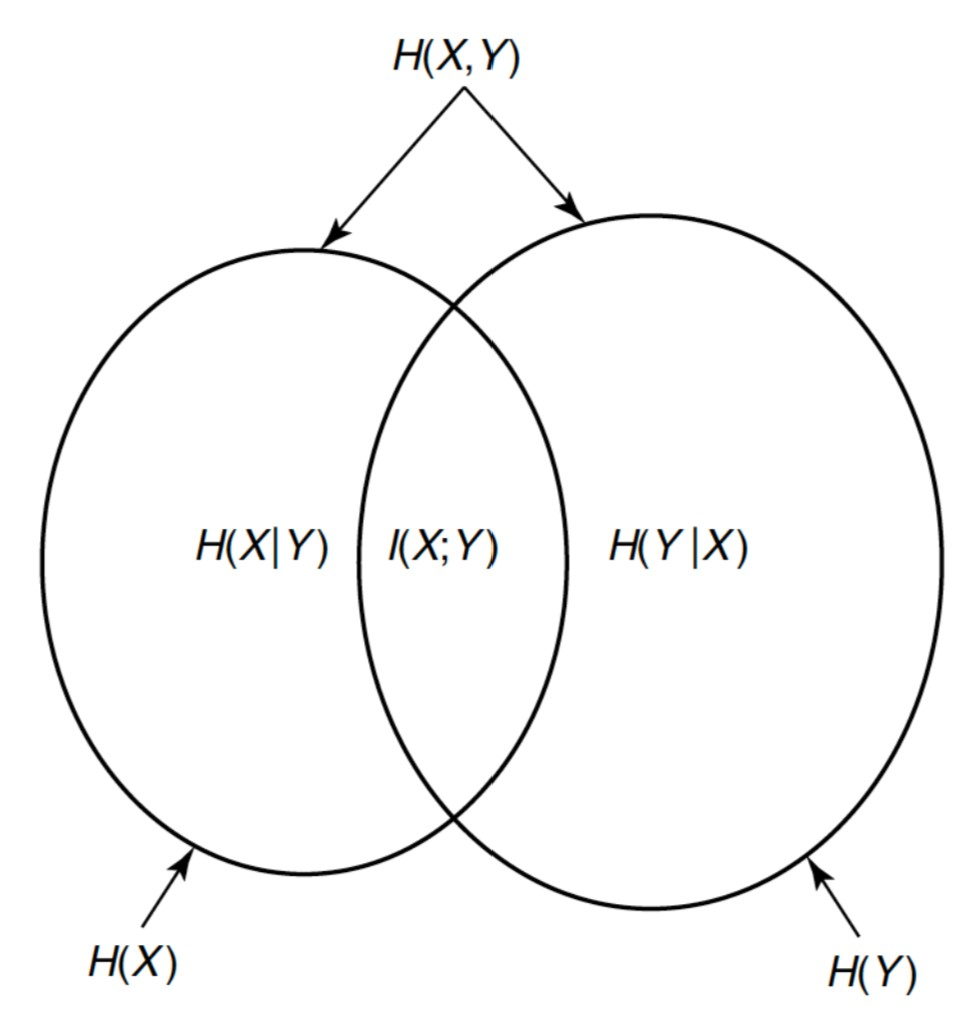
\includegraphics[scale = 0.5]{img/mutual information and entropy.jpg}
		\label{mi}
        \caption{Mutual information and entropy}
\end{figure}

\subsection{Data compression (source coding)}
In this section we introduce the notion of \textbf{source code}.

\image{img/sourceCoding}{Source coding theorem is focused on the first part of the channel.}{0.7}

As we introduced before, because of the presence of noise inside the channel, source and destination also have the task to ensure \textbf{efficiency} and \textbf{reliability} of messages. However, ensuring these two properties introduces another problem: \textbf{redundancy}. In order to achieve efficiency it is necessary to remove redundancy from the messages, using \textbf{compression}; on the other hand, improving reliability requires the receiver to be able to make inferences about the original message, which again can only be achieved through redundancy. As we can see there is an intrinsic \textbf{contrast} between the two requirements, hence it is necessary to find a good \textbf{trade-off}. A possible solution, for instance, is to send more (possibly an odd number of) bits to codify a single symbol (e.g. \verb|"0"| is encoded as \verb|"000"|). In this way the decoder will more easily be able to spot and fix errors in the received message, increasing reliability as well as redundancy.


Let $X$ be random variable with range $\mathcal{X}$:
$$\mathcal{X} = \{x_1, \cdots, x_n\}$$

and probability distribution

$$p(x) = Pr\{X=x\}$$

We define $\mathcal{D}$ as the channel alphabet and we define a code as a function that executes the following transformation:
$$C : \mathcal{X} \rightarrow \mathcal{D}^*$$
, where $\mathcal{D}^*$ represents the set of strings of symbols from the alphabet $\mathcal{D}$. In this sense, a code is a function that maps strings from the source code $\mathcal{X}$ to the channel code $\mathcal{D}$. We denote with $C(x)$ the \textbf{codeword} associated to $x$.

In general, it is clear that not all codes are good ones. However, there are some rules that can help us in order to define a good one:
\begin{itemize}
	\item It must be as \textbf{short} as possible in order to ensure the \textit{efficiency} of transmission.
	\item There must not be presence of codes that are prefixes of other ones: this leads problems with \textit{efficiency} because receiver must wait other bits in order to understand if sender has sent letter $\verb|"b"|$ or $\verb|"d"|$.
\end{itemize}  
It is also possible to have an efficient code that is useless, because receiver can't understand what is transmitted in the channel. An example is the following table in which \textbf{ambiguity} appears.
\begin{table}[H]
	\centering
	\begin{tabular}{| c | c |}
		\hline
		$\mathcal{X}$ & $\mathcal{D}^*$\\\hline
		$\verb|1|$ & $\verb|0|$ \\
		$\verb|2|$ & $\verb|0|$ \\
		$\verb|3|$ & $\verb|0|$ \\
		$\verb|4|$ & $\verb|0|$ \\
		\hline
	\end{tabular}
	\caption{Ambiguous code.}
\end{table}

\subsubsection{Classes of codes}
We can define the following classes of codes:

\begin{enumerate}
    \item \textbf{Non-singular codes}, in which all the codewords are distinct (i.e. the coding function $C$ is injective). Notice that non-singular codes can be not uniquely decodable, as represented below;

    \begin{table}[H]
	\centering
	\begin{tabular}{| c | c |}
		\hline
		$\mathcal{X}$ & $\mathcal{D}^*$\\\hline
		$\verb|1|$ & $\verb|0|$ \\
		$\verb|2|$ & $\verb|010|$ \\
		$\verb|3|$ & $\verb|01|$ \\
		$\verb|4|$ & $\verb|10|$ \\
		\hline
	\end{tabular}
	\caption{Example of non-singular but not uniquely decodable code.}
    \end{table}

    A code like this can generate a message such as $\verb|010|$, in which a decoder can generate more than one decoded message. For instance, it could generate 2, 14 or 31.. As we can see, even if we are in an optimal situation without noise, the receiver can't understand the message it received.

    \item \textbf{Uniquely decodable}, in which any encoded string must have a unique decoding. An example is provided here:

    \begin{table}[H]
	\centering
	\begin{tabular}{| c | c |}
		\hline
		$\mathcal{X}$ & $\mathcal{D}^*$\\\hline
		$\verb|1|$ & $\verb|10|$ \\
		$\verb|2|$ & $\verb|00|$ \\
		$\verb|3|$ & $\verb|11|$ \\
		$\verb|4|$ & $\verb|110|$ \\
		\hline
	\end{tabular}
	\caption{Example of uniquely decodable but not instantaneous code.}
    \end{table}

    \item \textbf{Instantaneous code} or \textbf{Prefix code}, in which no codeword is a prefix of any other. An example is provided here:

    \begin{table}[H]
	\centering
	\begin{tabular}{| c | c |}
		\hline
		$\mathcal{X}$ & $\mathcal{D}^*$\\\hline
		$\verb|1|$ & $\verb|0|$ \\
		$\verb|2|$ & $\verb|10|$ \\
		$\verb|3|$ & $\verb|110|$ \\
		$\verb|4|$ & $\verb|111|$ \\
		\hline
	\end{tabular}
	\caption{Example of instantaneous (or prefix) code.}
    \end{table}
    
\end{enumerate}

Notice that a uniquely decodable code is also non-singular (it is not always true the opposite), and an instantaneous/prefix code is also uniquely decodable: a scheme of the classes of codes is provided here:

\image{img/codesClassification}{Codes classification.}{0.7}

\subsection{Quantifying efficiency}
While we define a code, it is also useful to consider the efficiency given by it. If we consider a code like this:
\begin{table}[H]
	\center
\begin{tabular}{| c | c | c |}
	\hline
	$\mathcal{X}$ & $\mathcal{D}^*_1$ & $\mathcal{D}^*_2$\\\hline
	$\verb|a|$ & $\verb|0|$ & $\verb|0|$ \\
	$\verb|b|$ & $\verb|10|$ & $\verb|10001|$ \\
	$\verb|c|$ & $\verb|110|$ & $\verb|1100110|$ \\
	$\verb|d|$ & $\verb|111|$ & $\verb|1110010|$ \\
	\hline
\end{tabular}
\caption{Non-efficient code.}
\end{table}

, we can see immediately that the codewords use too many bits to codify the original symbol of the source. So we could consider the \textbf{length of codewords} as a \textbf{possible metric} to quantify efficiency of a code, but we will find out in the next example that this metric is not the best one.
\begin{exmp} Consider the following example:
	$$\mathcal{X} = \{a, b, c, d\} \qquad \mathcal{D} = \{0,1\}$$
	with the following probabilities:
	$$p(a) = \frac{1}{2} \qquad p(b) = \frac{1}{4} \qquad p(c) = \frac{1}{8} \qquad p(d) = \frac{1}{8}$$
	We can define two possible codes to convert symbols from $\mathcal{X}$ to $\mathcal{D}$.
	\begin{table}[H]
		\centering
		\begin{tabular}{| c | c | c |}
			\hline
			$\mathcal{X}$ & $\mathcal{D}^*_1$ & $\mathcal{D}^*_2$\\\hline
			$\verb|a|$ & $\verb|0|$ & $\verb|111|$ \\
			$\verb|b|$ & $\verb|10|$ & $\verb|110|$ \\
			$\verb|c|$ & $\verb|110|$ & $\verb|10|$ \\
			$\verb|d|$ & $\verb|111|$ & $\verb|0|$ \\
			\hline
		\end{tabular}
		\caption{Comparing codes.}
	\end{table}
\end{exmp}
The second code is the reversed version of the first one. If we consider only the length of the codewords we can say that in terms of efficiency they are equal, but this is not true. When we talk about efficiency, it is necessary to consider the probability distribution of the symbols. In this example the symbol $\verb|a|$ is very likely to appear, while symbol $\verb|d|$ is very unlikely to be found. In other words, while the second code maps $\verb|a|$ to a long codeword and $\verb|d|$ to a short one, the first code does the opposite, hence proving to be more efficient since it uses, on average, fewer bits.\\
We can thus define the \textbf{length of a code} with the following formula:
		$$ L(C) = \sum_{x \in \mathcal{X}} p(x) l(x) $$
, i.e. it is the average length of the codewords,
where $l(x)$ is the length of the codeword associated to the symbol $x$.

\begin{exmp} Let $X$ be a random variable with following range:
	$$\mathcal{X} = \{1, 2, 3, 4\} \qquad \mathcal{D} = \{0,1\}$$
	and the following probability distribution:
	$$p(X = 1) = \frac{1}{2} \qquad p(X = 2) = \frac{1}{4} \qquad p(X = 3) = \frac{1}{8} \qquad p(X = 4) = \frac{1}{8}$$

Then:

$$
L(C) = \frac{1}{2} \cdot 1 + \frac{1}{4} \cdot 2 + \frac{1}{8} \cdot 3 + \frac{1}{8} \cdot 3 = 1.75
$$

Notice that in this case $H(X) = 1.75 = L(C)$.

\end{exmp}

\begin{exmp} Let $X$ be a random variable with following range:
	$$\mathcal{X} = \{1, 2, 3\} \qquad \mathcal{D} = \{0,1\}$$
	and the following probability distribution:
	$$p(X = 1) = \frac{1}{3} \qquad p(X = 2) = \frac{1}{3} \qquad p(X = 3) = \frac{1}{3}$$

Then:

$$
L(C) = \frac{1}{3} \cdot 1 + \frac{1}{3} \cdot 2 + \frac{1}{3} \cdot 3 = 1.66
$$

However, in this case $H(X) = \log_2 3 = 1.58$ bits.

\end{exmp}

There is a theorem which states that entropy is a lower bound for $L(C)$, considering a \textbf{noise free channel}.

\begin{thm}[Shannon's theorem] 
	Let $X$ be a random variable (source), with range $\mathcal{X}$ and probability distribution $p(x)$. 
	Let $\mathcal{D}$ be the channel's alphabet, $C : \mathcal{X} \rightarrow \mathcal{D}^*$ an instantaneous code for X and $D = |\mathcal{D}|$.\\
	Then, if the channel is noise free: 
	$$ L(C) \geq H_D(X)$$
	where $D$ is the base of the logarithm. 
	
	Moreover:
	$$ L(C) = H_D(x) \iff \forall x \in \mathcal{X}: \quad l(x) = -\log_D p(x) = \log_D \frac{1}{p(x)} $$
\end{thm}

When the probability distribution $p(x)$ has the property:
$$ \log_D \frac{1}{p(x)} \in \mathbb{N}\setminus\{0\}$$
the probability distribution $p(x)$ is called \textbf{D-adic}. Thus, the equality in the theorem is reached if and only if the probability distribution is \textit{D-adic}.

\begin{exmp}
$$\mathcal{X} = \{a, b, c, d\} \qquad \mathcal{D} = \{0,1\}$$
with the following probabilities:
$$p(a) = \frac{1}{2} \qquad p(b) = \frac{1}{4} \qquad p(c) = \frac{1}{8} \qquad p(d) = \frac{1}{8}$$

$$ p(a) = \frac{1}{2} \quad \log_2 2 = 1$$
$$ p(b) = \frac{1}{4} \quad \log_2 4 = 2$$
$$ p(c) = \frac{1}{8} \quad \log_2 8 = 3$$
$$ p(d) = \frac{1}{8} \quad \log_2 8 = 3$$
\end{exmp}

\subsection{Huffman coding}
The \textbf{Huffman coding} is a \textbf{greedy algorithm} used to build/define the \textbf{best code} in a lossless data compression.

The algorithm proceeds as follows:

\begin{enumerate}
    \item Take the two least probable symbols in the alphabet. These two symbols will be given the longest codewords, which will have equal length, and differ only in the last digit;
    \item Combine these two symbols into a single one, and repeat.
\end{enumerate}

\begin{exmp} Huffman coding with $\mathcal{X} = \{x_1, \dots, x_6\}$ and $p(x) = (0.4,0.3,0.1,0.1,0.06,0.04)$.
	
	\begin{table}[H]
		\centering
		\begin{tabular}{| c | c | c | c | c | c | c | c | c | c | c |}
			\hline
			$\mathcal{X}$ & $p(x)$ & $c_5$ & $p(x)^1$ & $c_4$ & $p(x)^2$ & $c_3$ & $p(x)^3$& $c_2$ & $p(x)^4$&$c_1$ \\\hline
			$x_1$ & $0.4$ & $1$ & $0.4$ & $1$ & $0.4$ & $1$ & $0.4$& $1$ & $0.6$& $0$ \\
			$x_2$ & $0.3$ & $0$ & $0.3$ & $00$ & $0.3$ & $00$ & {\color{red}{*$0.3$}}& $00$ & $0.4$& $1$ \\
			$x_3$ & $0.1$ & $011$ & {\color{red}{*$0.1$}} & $011$ & {\color{red}{*$0.2$}} & $010$ & {\color{red}{*$0.3$}}& $01$ & &  \\
			$x_4$ & $0.1$ & $010$ & {\color{red}{*$0.1$}} & $0100$ & {\color{red}{*$0.1$}} & $011$ & & & & \\
			$x_5$ & {\color{red}{*$0.06$}} & $01010$ & $0.1$ & $0101$ & & & & & &\\
			$x_6$ & {\color{red}{*$0.04$}} & $01011$ &  &  &  & & & & & \\
			\hline
		\end{tabular}
		\caption{Comparing codes.}
	\end{table}
\end{exmp}

\begin{thm}[Optimality of Huffman codes]
    Huffman codes are optimal (and instantaneous).
\end{thm}

\begin{thm}
    If $C_{\text{Huffman}}$ is a Huffman $D$-ary code for a random variable $X$, then:

    $$
    H_D(X) \leq L(C_{\text{Huffman}}) < H_D(X) + 1
    $$
\end{thm}

\begin{exmp}
    Let $X$ be a r.v. with range $\mathcal{X} = \{ x_1, x_2 \}$ and $p(x_1) = \frac{2}{3}$ and $p(x_2) = \frac{1}{3}$. Then, the optimal (Huffman) code is :

    $$
    x_1 \xrightarrow{} 0
    $$

    $$
    x_2 \xrightarrow{} 1
    $$

    In this case, the length of the code is 1, and we can't apparently do better than this, but let's consider blocks of two consecutive symbols. Assuming statistical independence, we have $p(x_1, x_1) = \frac{4}{9}$, $p(x_1, x_2) = \frac{2}{9}$, $p(x_2, x_1) = \frac{2}{9}$, $p(x_2, x_2) = \frac{1}{9}$. An optimal (Huffman) code for this new source is :

    $$
    x_1 x_1 \xrightarrow{} 0
    $$

    $$
    x_1 x_2 \xrightarrow{} 10
    $$

    $$
    x_2 x_1 \xrightarrow{} 110
    $$

    $$
    x_2 x_2 \xrightarrow{} 111
    $$

    Now, the expected codeword length per input symbol is 0.944, which is less than before! Clearly, increasing the input size, we obtain better and better codes. Shannon's theorem states that this process will converge towards the entropy of $X$, in this case $H(X) = 0.91830$
    
\end{exmp}

\subsection{Channel}
In the previous sections, we covered the topic of coding. However, two different definitions of codes can be indicated:
\begin{itemize}
	\item \textbf{Lossless codes}, i.e. codes that don't lose any information from the initial source. It is possible to reconstruct completely the original message;
	\item \textbf{Lossy codes}, i.e. codes that lose information. After compression some information is lost (jpg, $\dots$).
\end{itemize}
Two meaningful concepts are \textbf{source coding}, which is related to \textit{efficiency}, and \textbf{channel coding}, that is, instead, related to \textit{reliability}. We will now focus exactly on this last topic. 

\subsubsection{Definition of channel}
A channel can be formally defined as a triplet:
$$\mathcal{C} = (\mathcal{X}, p(y|x), \mathcal{Y})$$
where:
\begin{itemize}
	\item $\mathcal{X}$ is the \textbf{input alphabet}.
	\item $p(y|x)$ is the \textbf{channel's probability distribution}. It represents the probability that symbol $x$ is translated into $y$. It is the most important component of the channel and it is defined as:
	$$p(y|x) = Pr(Y=y | X = x)$$
	\item $\mathcal{Y}$ is the \textbf{output alphabet}.
\end{itemize}
\image{img/channelDef}{Channel definition.}{0.6}

\subsubsection{Capacity of a channel}
Let us consider a channel $\mathcal{C}$, we want to analyze the mutual information $I(X;Y)$. We have defined the mutual information as:
$$I(X;Y) = H(X) - H(X|Y)$$
where:
\begin{itemize}
	\item $H(X)$ is considered as $f(p(x))$ function of the probability distribution of the source.
	\item $H(X|Y) = -\sum_x \sum_y p(x,y) \log{p(x|y)}$, where:
		\begin{itemize}
			\item $p(x,y) = p(x)p(y|x)$ in which $p(x)$ is related to the \textit{source} and $p(y|x)$ is related to the \textit{channel}. Generally, it is possible to say that $p(x,y)$ depends both on the source and on the channel.
			\item From Bayes Theorem we also know that $$p(x|y) = \frac{p(y|x) p(x)}{p(y)}$$ in which again $p(y|x)$ is related to the \textit{channel} and instead $p(x)$ is related to the \textit{source}.
			$$p(y) = \sum_x p(x,y) = \sum_x \underbrace{p(x)}_{source}\underbrace{p(y|x)}_{channel}$$
		\end{itemize} 
\end{itemize}
The mutual information that travels on the channel depends both on the source and on the channel.
$$I(X;Y) = f(p(x), p(y|x)) = f(source, channel)$$
where:
\begin{itemize}
	\item $p(x)$ is the ``a priori''  probability.
	\item $p(y|x)$ is the ``a posteriori'' probability.
\end{itemize}
This means that we can't use mutual information to give capacity information of the channel since $I(x,y)$ is not only dependent on the channel itself, but also on the source.	
After all these premises, we are able to define the \textbf{capacity of channel} as:
$$C = \max_{p(x)} I(X;Y)$$

The \textbf{capacity} represents the maximum value of mutual information given by all the possible probability distributions of the source. 
\begin{exmp}
	We compute the capacity of the following Binary Symmetric Channel:\\
	\image{img/exampleCapacity}{Binary symmetric channel.}{0.6}
	We know that $P\{X=0\} = \pi$ and $P\{X=1\} = 1-\pi$ (with $\pi \in [0,1]$).

What could happen in the different extreme cases is explained in the following lines:
\begin{itemize}
	\item $p = 0$, we have that the channel is \textbf{perfect} and its capacity is 1. This represent the ideal case in which the channel is not affected by noise and receiver knows that the messages are correct. No loosing of information.
	\image{img/p0}{Channel representation when $p=0$.}{0.3}
	
	\item $p = 1$, we have that the channel is again \textbf{perfect}. Receiver always knows how to reconstruct the right message. The message is always modified during the transmission on the channel. The channel's capacity is again 1.
	\image{img/p1}{Channel representation when $p=1$.}{0.3}
	
	\item $p=0.5$ is the worst scenario for the receiver. We can consider the starting message $X$ and the final message $Y$ as independent messages.
	\image{img/p05}{Channel representation when $p=0.5$.}{0.3}
\end{itemize}
\end{exmp}
Here there is a strong assumption: the \textbf{receiver knows the probability distribution of the channel.}
The best case for the receiver is to know both the channel distribution and the sender distribution, but this is not always feasible.
Probabilities of the channel, in fact, can be specified only after several trials and they are not fixed, as they could change during the time.

\subsection{Reliability}
When we have a noisy channel, the simplest way to improve reliability is exploit the \textbf{repetition of the code}, i.e. add redundancy to the code, in order to reduce the probability of errors during the communication.

\begin{figure}[h!]
		\centering
        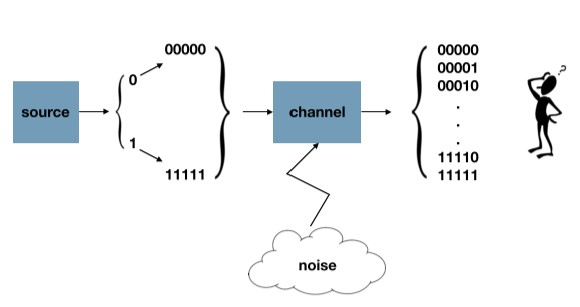
\includegraphics[scale = 1.5]{img/redundancy.jpg}
		\label{mi}
        \caption{Adding redundancy in a noisy channel}
\end{figure}

Notice that in this case the receiver decides how to decode the redundant message by taking, for example, a majority vote. Assume that a channel is BSC with error probability $p = 10^{-2}$. Then, using a repetition code of length 3, we reduce this error probability to $3 \cdot 10^{-4}$, but at the same time we reduced the transmission rate to $\frac{1}{3}$.

If we use a repetition code of length 5, we reduce the probability of error to approximately $10^{-5}$, reducing the transmission rate to $\frac{1}{5}$.

What if we now consider $n \rightarrow \infty$? Let's define $P_e$ as the error probability. When $n \rightarrow \infty$ we have that $P_e \rightarrow 0$ but $R \rightarrow 0$, meaning that a more reliable code produces a slower communication system.
It is necessary to find a right trade-off to maintain a good level of reliability and speed.

\subsection{Channel coding theorem - Shannon's 2nd theorem}
\begin{thm}[Channel coding theorem]
	Let $\mathcal{C}$ be a channel with capacity $C$.
	\begin{itemize}
		\item If $R < C$, there exists a sequence of codes with transmission rate $R$ such that:
		$$P_e  \underset{n \rightarrow \infty}{\rightarrow} 0$$

        \item Conversely, if a sequence of codes transmitting at rate $R$ has a probability error approaching to zero (i.e. $P_{e} \rightarrow 0$), then $R \leq C$. 
        \end{itemize}
\end{thm}

In this sense, this theorem states that we can send a message \textbf{at a finite rate} through a noisy channel with error probability \textbf{as small as we want}, provided that we transmit at a rate smaller than the capacity. Thus, the \textbf{capacity} of the channel is an \textbf{upper bound} for $R$ if we want to define a reliable code.
